\documentclass{amia}
\usepackage{graphicx}
\usepackage[labelfont=bf]{caption}
\usepackage[superscript,nomove]{cite}
\usepackage{color}
\usepackage{soul}
\usepackage{multirow}
\usepackage{url}
\renewcommand*{\thefootnote}{\alph{footnote}}

\begin{document}

\title{Deep Neural Architectures for Discourse Segmentation in E-Mail Based Behavioral Interventions}

\author{Mehedi Hasan, BS$^{1}$\footnote{Authors provided an equal contribution. \label{footnote1}}, Alexander Kotov, PhD$^{1}$\textsuperscript{\ref{footnote1}}, Sylvie Naar, PhD$^{2}$, Gwen L. Alexander, PhD$^{3}$, April Idalski Carcone, PhD$^{4}$}

\institutes{
$^1$Department of Computer Science, Wayne State University, Detroit, Michigan \\  
$^2$Center for Translational Behavioral Research, Department of Behavioral Sciences and Social Medicine, Florida State University, Tallahassee, Florida\\
$^3$Department of Public Health Sciences, Henry Ford Health System, Detroit, Michigan\\
$^4$Department of Family Medicine and Public Health Sciences, School of Medicine, Wayne State University, Detroit, Michigan\\
}

\maketitle

\noindent{\bf Abstract}
\textit{Communication science approaches to develop effective behavior interventions, such as motivational interviewing (MI), are limited by traditional qualitative coding of communication exchanges, a very resource-intensive and time-consuming process. This study focuses on the analysis of e-Coaching sessions, behavior interventions that are delivered via email and grounded in the principles of MI. A critical step towards automated qualitative coding of e-Coaching communication exchanges is segmentation of emails into fragments that correspond to MI behaviors. This study frames email segmentation task as a classification problem and utilizes word embeddings in conjunction with punctuation and part-of-speech features to address it. We experimentally evaluated conditional random fields (CRF), a traditional machine learning method, as well as deep learning methods, such as multilayer perceptron (MLP), bidirectional recurrent neural network (BRNN) and convolutional recurrent neural network (CRNN). Our results indicate that CRNN outperform CRF, MLP and BRNN for the task of email segmentation achieving 0.989 macro F1-score overall and 0.825 macro F1-score for new segment detection.}

\section*{Introduction}
The emergence of e-Health technologies has greatly expanded the reach of behavioral interventions. One such intervention is email-delivered Motivational Interviewing (MI). MI is an evidence-based communication technique to increase intrinsic motivation and self-efficacy for behavior change\cite{miller2012motivational,miller2009toward}. MI is linked to behavior change through the elicitation of patient ``change talk'', or statements of intrinsic motivation expressing patients’ own desires, abilities, reasons, need for, and commitment to behavior change\cite{apodaca2009mechanisms}. However, communication science approaches to understanding the efficacy of MI are inherently limited by traditional qualitative coding methods. The specific provider behaviors responsible for the elicitation of change talk, however, are less clear and may vary by treatment context. Thus, a current focus of MI research is understanding which provider behaviors in which contexts lead to patient change talk. To date, no study has examined this process in email-delivered MI.

The study of patient-provider communication in MI relies on the behavioral coding of intervention transcripts, an iterative, resource-intensive, and cognitively demanding process of qualitative analysis involving several iterations of reading, comprehension and interpretation of interview transcripts. Rapidly developing computational technologies, specifically, machine learning methods, offer an opportunity to dramatically accelerate this process. In particular, machine learning methods have been successfully applied to a variety of analytical tasks involving textual data, such as classification\cite{nigam2000text} and sentiment analysis.\cite{wang2012baselines} In our previous work, we examined the utility of machine learning methods for automated annotation \cite{hasan2016study,kotov2015interpretable} and predicting the outcome \cite{hasan2018predicting} of in-person MI sessions. Experimental data utilized in these studies were transcribed auto recordings of in-person MI sessions with a counselor, which were segmented into counselor and client utterances during the transcription process. 

In this study, we focus on the analysis of email-delivered MI, or e-Coaching, to promote healthy eating among young adults. The e-Coaching dataset is composed of email correspondence between a MI counselor and the young adult patient. Unlike transcribed in-person discourse, email correspondence is not clearly segmented into codable speech acts (i.e., utterances). Thus, the unstructured nature of e-Coaching exchanges poses a unique set of analytic challenges. Segmentation of e-Coaching exchanges into textual fragments that correspond to distinct e-Coach and patient communication behaviors is a significant barrier to qualitative analysis of this type of clinical conversation. Automating this task is a unique and challenging problem due to the following reasons:

\begin{enumerate}
\item Emails are unstructured text containing informal information exchange in a non-traditional format. For example, an e-Coach usually responds to several previous patient statements in one email. In contrast, in a traditional, in-person MI session, an utterance is assumed to be a response to the immediately preceding utterance.
\item Discourse segments in e-Coaching do not have a clear breakpoint, such as the end of a sentence or paragraph. One sentence might be divided into fragments corresponding to multiple MI behaviors. On the other hand, an MI behavior may comprise several sentences.
\end{enumerate}

\begin{figure}[!htb]
    \centering
    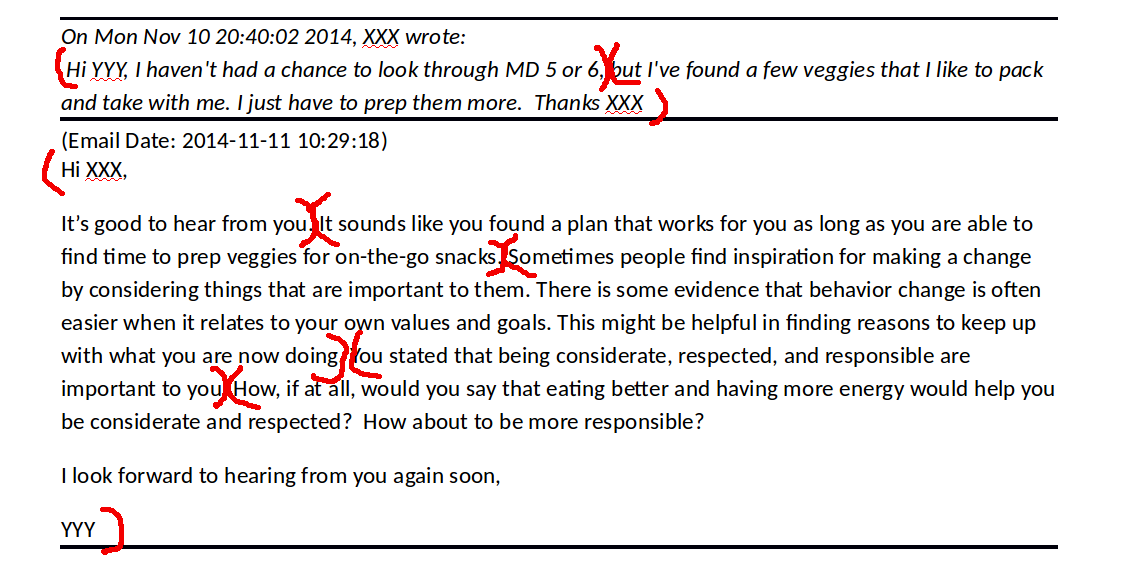
\includegraphics[width=0.7\textwidth]{figures/segment-example.png}
    \caption{\textbf{Example of an e-Coaching exchange segmented into fragments corresponding to MI behaviors of an e-Coach and a patient}}
    \label{fig:text-segment}
\end{figure}

Figure~\ref{fig:text-segment} illustrates a segmentation of an e-Coaching exchange, in which the first sentence is segmented into 2 MI behavior fragments, while the fourth and fifth segments correspond to one and three sentences, respectively. Segmentation of e-Coaching exchanges constitutes a special case of clinical discourse analysis \cite{webber2012discourse} aimed at better understanding the effective communication strategies specific to this type of behavioral interventions. 

The goal of this study is to assess the effectiveness of deep learning methods for the task of automated segmentation of e-Coaching emails into textual fragments corresponding to individual patient and provider behaviors.  For this study, we utilized the data from MENU GenY (Making Effective Nutrition Choices for Generation Y) \cite{alexander2017motivations}, a web-delivered public health intervention with email-based coaching to encourage increased fruit and vegetable intake among young adults, aged 21–-30. A secondary goal of the MENU GenY project was to identify the specific communication strategies used by e-Coaches to elicit change talk for healthier eating among young adult patients. Segmentation of clinical conversation in the context of electronically delivered interventions into groups of MI behaviors, is traditionally performed manually by MI researchers, which significantly slows down their qualitative analysis. This paper is the first work to evaluate the empirical effectiveness of deep learning architectures in addressing \textit{the problem of discourse segmentation in the context of e-mail-based behavioral interventions}. 

Specifically, we introduce and evaluate the effectiveness of distributed word representations (i.e. word embeddings) as well as lexical, punctuation and part-of-speech (POS) features in conjunction with both traditional supervised machine learning methods, such as linear-chain Conditional Random Fields (CRF)\cite{lafferty2001conditional} and deep learning methods, such as Multi-Layer Perceptron (MLP),\cite{rumelhart1986learning} Bidirectional Recurrent Neural Network (BRNN)\cite{schuster1997bidirectional} and Convolutional Recurrent Neural Network (CRNN),\cite{treviso2017sentence} to find the best performing method and feature combination. 

\section*{Related work}

Prior work on textual segmentation in the biomedical domain primarily focused on sentence boundary detection \cite{griffis2016quantitative,kreuzthaler2015detection,treviso2017sentence} and segmentation of clinical documents in patients' electronic health records (EHR) into sections and headers. \cite{apostolova2009automatic,denny2009evaluation,tepper2012statistical,cho2002text} In particular, Maximum Entropy models \cite{tepper2012statistical} and Support Vector Machine (SVM) along with word-vector cosine similarity metric and several heuristics \cite{apostolova2009automatic} have been applied to identify specific sections in EHR, such as general patient information, medical history, procedures, findings, etc. Denny et al. \cite{denny2009evaluation} proposed SecTag algorithm, which combined natural language processing techniques, terminology-based rules and a Na\"{i}ve Bayes classifier to identify sections and headers in EHR. Segmentation of e-Coaching emails, however, is different from segmentation of other clinical documents, since the focus is on dialog acts in clinical conversation.   

SVM in conjunction with prosodic and part-of-speech features \cite{kreuzthaler2015detection} and Recurrent Convolutional Neural Networks \cite{griffis2016quantitative} have also been utilized for \textit{sentence boundary detection} in general text. Liu et al. \cite{liu2005using} demonstrated that a linear-chain CRF outperforms Hidden Markov and Maximum Entropy models for this task. 

Segmentation of e-Coaching emails is also different from traditional shallow discourse analysis \cite{galley2003discourse}, which besides identification of speech acts, also aims to determine the types of transitions between speech acts and labels speech acts with speakers who performed them in a multi-speaker conversation. The proposed methods will automate the process of segmenting clinical exchanges into MI behaviors, which will significantly reduce the time and resources required to perform such segmentation manually. Furthermore, these methods can be integrated with auto coding methods \cite{hasan2016study,kotov2015interpretable} to create a software pipeline for fully automated analysis of email-delivered behavioral interventions.
  
\section*{Materials and methods}
\subsection*{\textit{Data collection}}
The experimental dataset for this work was constructed from 49 e-Coaching sessions, which include 330 and 281 emails by e-Coaches and patients, respectively. Various statistics of experimental dataset are provided in Table~\ref{tab:datastat}. Each session represents an MI intervention delivered via email. Emails were segmented into 3,138 text fragments and and annotated using the Minority Youth-Sequential Coding of Process Exchanges (MYSCOPE),~\cite{carcone2013provider} a qualitative coding scheme to characterize patient-provider communication during MI sessions with 115 distinct behavior codes. We consider email segmentation as a binary classification problem, in which each word or punctuation mark is annotated with a class label ``new segment'' or ``same segment'' to indicate whether it precedes a new segment or not. In total, the dataset consists of 95,777 words and 7,140 punctuation marks and includes 3,138 ``new segment'' and 99,779 ``same segment'' instances. In this study, we experimented with traditional machine learning methods, such as Conditional Random Fields (CRF)\cite{lafferty2001conditional} and deep learning methods, such as Multi-Layer Perceptron (MLP),\cite{rumelhart1986learning} Bidirectional Recurrent Neural Network (bidirectional RNN or BRNN)\cite{schuster1997bidirectional} and Convolutional Recurrent Neural Network (CRNN).\cite{treviso2017sentence} For an MLP model, training and testing samples were created based on a sliding window of $2n$ words or punctuation marks over each position (which could be a word or a punctuation mark) in a given input sequence, such that each instance consists of the $n$ words or punctuation marks after this position and $n$ words or punctuation marks prior to this position, including the position itself. Each sample is assigned a ``new segment'' or ``same segment'' label based on whether there should be a segment break after the current position or not. In the case of CRF, BRNN and CRNN models, an e-Coaching email was taken as an input sequence, POS tags and word embeddings of each word or punctuation mark were used as input and binary labels corresponding to ``new segment'' and ``same segment'' classification decisions were considered as the model output. In the gold standard, words or punctuations within the same segment were assigned the label of 0 and the last word or punctuation mark of a segment were assigned the label of 1 (an example of a sequence with assigned labels is provided in the $2^{nd}$ row of Table~\ref{tab:datastat}). \\ 

\begin{table}[ht]
\centering
\caption{\textbf{Summary of statistics of experimental dataset.}}
\label{tab:datastat}
 \begin{tabular}{|l|l|l|l|l|l|l|l|l|l|}
  \hline
   \multirow{2}{*}{\textbf{Sessions}} & \multirow{2}{*}{\textbf{Instances}} & \multicolumn{2}{|c|}{\textbf{Class Segments}} & \multicolumn{2}{|c|}{\textbf{Tokens}} & \multicolumn{2}{|c|}{\textbf{Emails}} & \multicolumn{2}{|c|}{\textbf{Annotation}} \\\cline{3-10}
   &  & \textbf{new}  & \textbf{same} & \textbf{words} & \textbf{punctuations}  & \textbf{patient} & \textbf{provider} & \textbf{method}  & \textbf{codes} \\ \hline    
 49 & 102,917 & 3,138 & 99,779 & 95,777 & 7,140 & 281 & 330 & MYSCOPE & 115 \\ \hline
 \multicolumn{10}{|c|}{segmentation example: Hi[0] XXX[0] ,[0] its[0] good[0] to[0] hear[0] from[0] you[0] .[1] it[0] sounds[0] like[0]...} \\ \hline
  \end{tabular}
\end{table}     

\subsection*{\textit{Features}}
We utilized three types of features in conjunction with CRF, MLP, BRNN and CRNN methods: word embeddings as lexical features, punctuation and POS features. Syntactic abstractions of individual words, such as POS tags, have been previously shown to be effective features for similar natural language processing tasks.\cite{liu2005using,treviso2017sentence} To extract POS features, we pre-processed e-Coaching emails using the NLTK POS tagger\footnote{\url{https://www.nltk.org/}}. Punctuation marks, which correspond to one of the symbols \{`.', `,', `!', `?', `:', `;'\} between a pair of words, were also used as a feature, since punctuation marks designate the boundary of a sentence, clause or phrase and often also correspond to a segment boundary.\cite{cho2002text} For natural language processing (NLP) tasks, inputs are received as a text, in which individual words are as the basic lexico-semantic units. Therefore, it is important to represent a word in such a way that preserves all relevant lexical and semantic information. Dense real-valued vector (i.e. embedding) is a form of distributed word representation, in which each word is associated with a vector in a low-dimensional vector space. Embeddings have been previously shown to effectively capture semantic, syntactic and morphological properties of words.\cite{pennington2014glove, mikolov2013distributed} For experiments reported in this paper, we utilized word embeddings pre-trained on Google News corpus consisting of 1.6 billion words using word2vec software package.\footnote{\label{fn:word2vec}https://code.google.com/p/word2vec/} For words or punctuation marks, which do not have pre-trained embeddings, we utilized the embeddings of the same dimensionality trained on the experimental dataset. CRF utilized lexical features, POS tags and the preceding label. 

\subsection*{\textit{Methods}}

We experimented with 4 different classifiers, including one traditional machine learning model (CRF) and three deep learning methods (MLP, BRNN and CRNN). Since deep learning architectures provide a flexible mechanism for constructing complex models, we take advantage of this flexibility to test different variations of MLP, BRNN and CRNN models for the task of segmentation of e-Coaching emails.

\textbf{Conditional Random Field}: CRF has been widely used in various sequence annotation NLP tasks, such as part-of-speech tagging.\cite{lafferty2001conditional, hirohata2008identifying} Unlike a maximum entropy Markov model, which uses per-state exponential models for conditional probability of the next state given a current state, CRF model directly estimates a distribution of the entire output sequence conditioned on the observation sequence. A traditional linear-chain CRF model is defined as a conditional probability distribution $p(y|x)$ of output sequence $y$, given input sequence $x$:

\begin{equation}
\label{Eq:crf}
p(y|x) = \frac{1}{Z_x}\exp{\left(\sum_{t=1}^{T}\sum_{k}^{}\lambda_k f_k(y_{t-1}, y_t, x, t)\right)} \\
\end{equation}

where $Z_x$ is a normalization factor, $f_k(y_{t-1}, y_t, x, t)$ is a feature function, and $\lambda_k$ is a learned weight associated with feature $f_k$. The optimal output sequence $y^*$ for input sequence $x$, $y^* = {arg\,max}_y p(y|x)$, is obtained efficiently using the Viterbi algorithm. In our experiments, the following features were utilized in conjunction with CRF models: i) current word or punctuation ii) next and previous 3 words or punctuations iii) binary feature indicating whether a word or punctuation is a special character (';', '?', '.', ',', '!', ':', etc.) or not iv) binary feature indicating whether a word is a title word or not (e.g. ``The'' is a title word but ``the'' is not) v) POS tags.   

\textbf{Multi-Layer Perceptron}: MLP is a neural network, which consists of multiple fully connected layers that map an input onto one or several outputs.\cite{rumelhart1986learning} Figure~\ref{fig:mlp} illustrates a multi-layer perceptron with a single hidden layer. MLPs have no cycles or loops. Information in them flows only forward, from the input layer through the hidden layer(s) to the output layer. The MLP in this study utilizes one hidden layer consisting of 128 neurons and rectified linear unit (ReLU) as a nonlinear activation function. In order to prevent over-fitting, we applied dropout (random masking of neurons) \cite{srivastava2014dropout} to fully connected layers during training. Dropout was also applied to fully connected layers in BRNN and CRNN. 

\begin{figure}[!htb]
    \centering
    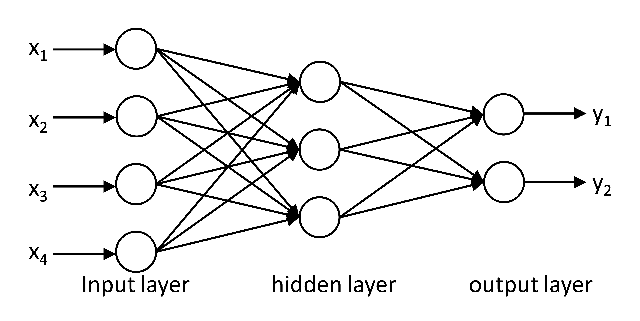
\includegraphics[width=0.45\textwidth]{figures/mlp.eps}
    \caption{\textbf{Multi-layer perceptron with a single hidden layer}}
    \label{fig:mlp}
\end{figure}

\textbf{Bidirectional Recurrent Neural Network}: BRNN is a neural network designed to capture sequential patterns by considering both past  and future inputs as well as complex relationships between input features and output labels.\cite{schuster1997bidirectional} The hidden state of BRNN is an aggregation of the hidden states of a forward and backward recurrent neural networks (RNNs). Gated Recurrent Units (GRU)\cite{chung2014empirical} capable of handling variable size input sequence and having internal memory, which can be reset, were utilized as an RNN. %Figure~\ref{fig:crnn} represents the architecture of BRNN, in the case when a convolution layer is removed.   

\textbf{Convolutional Recurrent Neural Network}: CRNN \cite{treviso2017sentence} shown in Figure~\ref{fig:crnn} is a deep neural network architecture, which combines convolutional and recurrent layers. Our implementation of CRNN consists of 5 layers: 1) input layer 2) embedding layer 3) convolution layer with max pooling 4) BRNN layer 5) fully connected layer with dropout and sigmoid output. E-coaching email exchanges are represented as a sequence of $m$ words and punctuations, which are fed into the input and embedding layers to produce a $m \times n_e$ matrix after fetching the embeddings for words and punctuations in the input sequence. This matrix corresponds to the distributed representation of an input email exchange, which contains rich morpho-syntactic information that can be utilized for its segmentation. When POS tags are utilized along with word embeddings, they are represented with a 10-dimensional vector, which is concatenated with 300-dimensional word embeddings to obtain new embedding vectors $n_e = [n_w;n_p]$ of size 310. The primary purpose of a convolution layer is to extract new features for each word or punctuation mark based on the neighboring words or punctuation marks. A one-dimensional (1D) convolution operation is utilized in this layer in our implementation of BRNN. In 1D convolution, one filter is responsible for extraction of one feature. After applying $n_f$ different filters with zero-padding on both sides of the input text, $n_f$ features are produced by the convolution layer for each word. A max pooling over time operation was then performed to find the most significant features in a textual fragment. The bidirectional recurrent layer receives new features extracted by the convolution layer. Unidirectional RNNs are usually used to capture long-range dependencies in a sequence of observations. Bidirectional RNNs, on the other hand, are capable of capturing both past and future contexts through forward and backward traversals of a sequence. The purpose of the fully connected layer is to use the output of the bidirectional RNN layer for classifying each word or punctuation into ``new segment'' or ``same segment'' classes. Since a fully connected layer has a larger number of parameters, they are more likely to excessively co-adapt to  other parameters, which may result in over-fitting. To prevent this, we utilized dropout by randomly ignoring 50\% of the connections in the fully connected layer. Finally, logistic sigmoid outputs the probability of classifying or labeling each word or punctuation mark with ``same segment'' class. We experimentally determined the optimal parameters using 5-fold cross-validation and found out that the best performance is achieved when filter length in the convolution layer is 7, number of filters is 100, max-pool size is 3, ReLU is used as an activation function in the convolution layer, hyperbolic tangent is used as an activation function in the bi-directional RNN layer and the number of dimensions in the hidden state of RNNs is 200. Adam\cite{kingma2014adam} with 50 epochs, the batch size of 32 and learning rate of 0.001 was used for optimization and the early stopping strategy was applied.\footnote{source code of all methods is available at \url{https://github.com/teanalab/eCoaching-Text-Segmentation}}

\begin{figure}[!htb]
    \centering
    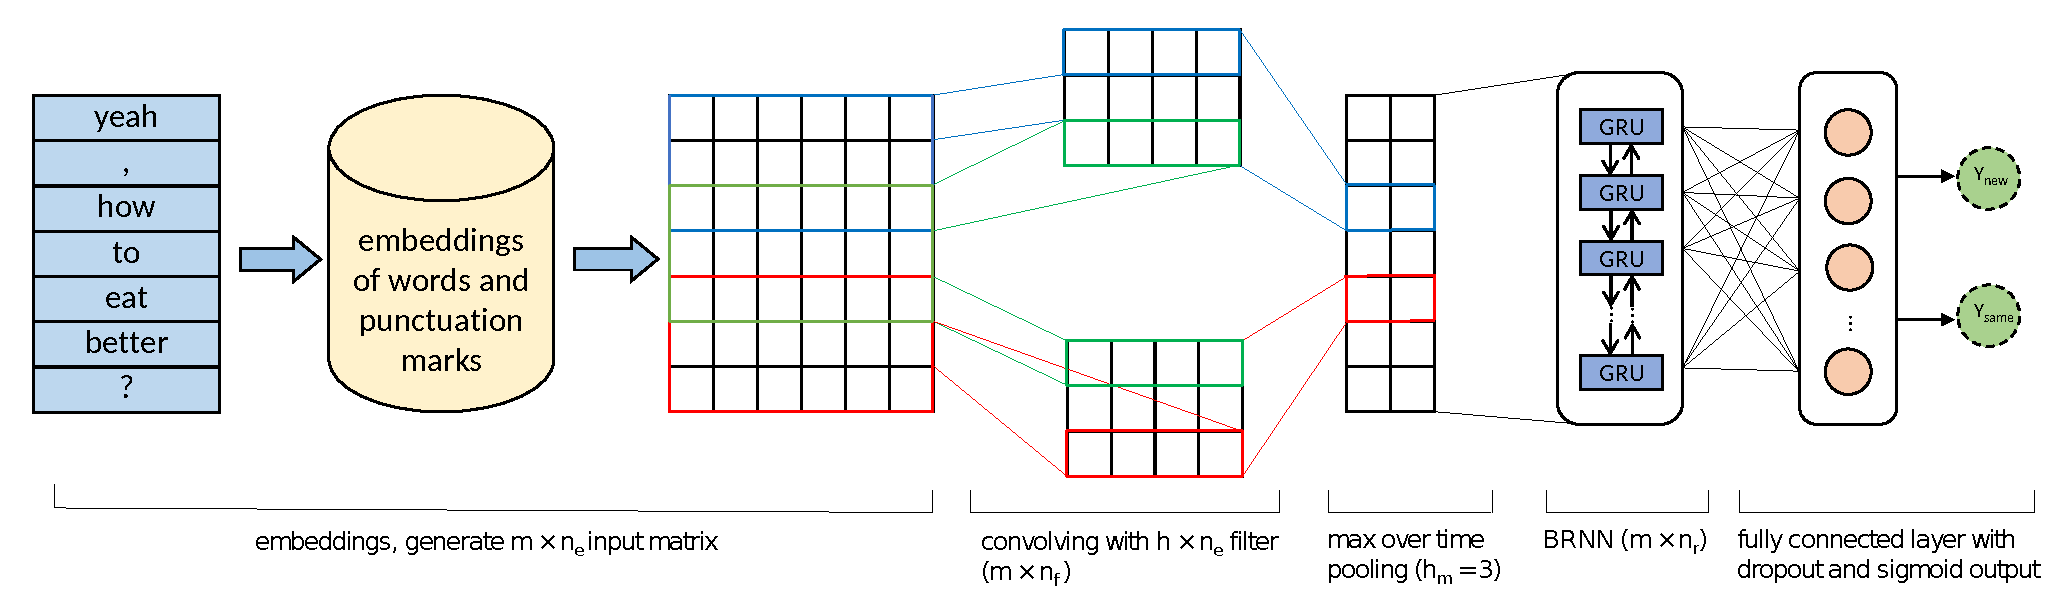
\includegraphics[width=0.95\textwidth]{figures/CRNN.eps}
    \caption{\textbf{Architecture of a convolutional recurrent neural network for automated segmentation of e-Coaching emails}}
    \label{fig:crnn}
\end{figure}
  
\subsection*{\textit{Evaluation metrics}}
We report standard metrics of precision, recall and F1-measure to evaluate the performance of the classifiers.\cite{aas1999text} Accuracy is not reported as a performance metric, since it is highly sensitive to the prior class probabilities and does not fully describe the actual difficulty of the decision problem, when highly unbalanced datasets are involved. The results are reported based on 5-fold cross-validation (one fold was used as a test set and the remaining 4 folds were utilized as a training set) and weighted macro-averaging over the folds. We also report the area under the precision-recall curve (AUPR), due to its effectiveness in measuring the performance of binary classifiers in the case of the datasets with imbalanced class distribution.\cite{davis2006relationship}

\section*{Results}
Our experiments spanned three dimensions. First, we determined the optimal size of word embedding vectors and the sliding window of MLP. Second, we evaluated the performance of different methods with respect to detecting ``new segment'' as well as the weighted average over ``new segment'' and ``same segment'' classes. Third, we assessed the impact of different types of features as well as their combination on the performance of different machine learning methods on the e-Coaching email segmentation task.

\begin{figure}[!htb]
    \centering
    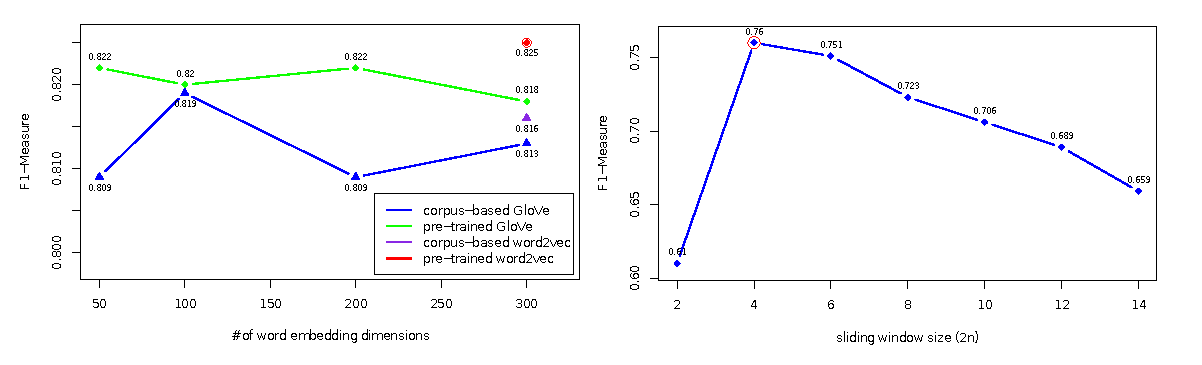
\includegraphics[width=0.95\textwidth]{figures/mlp-and-vector.eps}
    \caption{\textbf{F1-measure of CRNN on the task of e-Coaching email segmentation by varying the number of dimensions in pre-trained and corpus-based GloVe and word2vec embeddings (left). F1-measure of MLP on the task of e-Coaching email segmentation by varying the size of the sliding window (right).}}
    \label{fig:embedding-dimension-mlp}
\end{figure}   

Figure~\ref{fig:embedding-dimension-mlp} (left) illustrates the performance of CRNN on the task of e-Coaching email segmentation by varying the number of dimensions in pre-trained and corpus-based GloVe \footnote{https://nlp.stanford.edu/projects/glove/} and word2vec embeddings. We observed that the best performance is achieved with pre-trained 300-dimensional word2vec word vectors, when three types of features are used together. Therefore, we report the results for other deep learning models used in this study when 300-dimensional word2vec embedding vectors are utilized. The input layer of MLP consists of a sum of embeddings of $n$ words or punctuation marks before and the sum of embeddings of $n$ words or punctuation marks after the word or punctuation mark, which is the center of a sliding window of $2n$ words or punctuation marks. Figure~\ref{fig:embedding-dimension-mlp} (right) demonstrates the performance of MLP on e-Coaching email segmentation by varying the size of the sliding window. It can be observed that the best performance of MLP is achieved when the size of the sliding window is 4 (or $n=2$). Therefore, MLP results in the remaining experiments are reported when $n$ is set to 2.

\begin{table}[ht]
\centering
\caption{\textbf{Performance of CRF, MLP, BRNN and CRNN on ``new segment'' detection as well as the weighted average over ``new segment'' and ``same segment'' classes when only lexical features are used. The highest value for each performance metric is highlighted in boldface.}}
\label{tab:result_base}
  \begin{tabular}{|l|l|l|l|l|l|l|}
  \hline
   \multirow{2}{*}{\textbf{Method}} & \multicolumn{3}{|c|}{\textbf{New Segment}} & \multicolumn{3}{|c|}{\textbf{Overall}} \\\cline{2-7}
   & \textbf{Precision}  & \textbf{Recall} & \textbf{F1-Measure} & \textbf{Precision}  & \textbf{Recall} & \textbf{F1-Measure} \\ \hline    
 CRF & 0.782 & 0.691 & 0.733 & 0.983 & 0.984 & 0.984 \\ \hline
 MLP & \textbf{0.836} & 0.593 & 0.694 & 0.982 & 0.983 & 0.982 \\ \hline
 BRNN & 0.606 & 0.680 & 0.641 & 0.977 & 0.976 & 0.976 \\ \hline
 CRNN & 0.775 & \textbf{0.797} & \textbf{0.785} & \textbf{0.986} & \textbf{0.986} & \textbf{0.986} \\ \hline
  \end{tabular}
\end{table}                              

As follows from Table~\ref{tab:result_base}, CRNN outperforms all other methods in terms of recall and F1-measure achieving 0.797 recall and 0.785 F1-measure for new segment detection. CRNN also shows superior performance according to all performance metrics calculated as a weighted average over ``new segment'' and ``same segment'' classes. BRNN demonstrates the lowest performance among all models in terms of precision and F1-measure. On the other hand, MLP demonstrated the highest precision of 0.836 when word embeddings or lexical features are used to identify ``new segment''. CRF achieves 0.733 F1-measure on new segment detection and 0.984 F1-measure overall, which corresponds to the second highest performance in identifying ``new segment''. CRF also demonstrated the second highest performance according to all metrics calculated as a weighted average over both classes. Experimental results indicate that the performance of all classifiers according to all metrics calculated as a weighted average over both classes is significantly higher than their performance on ``new segment'' detection, which is expected since 96.95\% of instances belong to the ``same segment'' class and 99.3\% of them are correctly classified. For example, CRNN achieves 27.23\%, 23.71\% and 25.61\% higher precision, recall and F1-measure calculated as a weighted average over ``new segment'' and ``same segment'' classes, compared to the ``new segment'' detection. \\

\begin{table}[ht]
\centering
\caption{\textbf{Performance of CRF, MLP, BRNN and CRNN on ``new segment'' detection as well as the weighted average over ``new segment'' and ``same segment'' classes when all types of features are used together. The highest value for each performance metric is highlighted in boldface.}}
\label{tab:result_weighted_avg}
 \begin{tabular}{|l|l|l|l|l|l|l|}
  \hline
   \multirow{2}{*}{\textbf{Method}} & \multicolumn{3}{|c|}{\textbf{New Segment}} & \multicolumn{3}{|c|}{\textbf{Overall}} \\\cline{2-7}
   & \textbf{Precision}  & \textbf{Recall} & \textbf{F1-Measure} & \textbf{Precision}  & \textbf{Recall} & \textbf{F1-Measure} \\ \hline    
 CRF & 0.813 & 0.772 & 0.792 & 0.988 & 0.988 & 0.988 \\ \hline
 MLP & \textbf{0.817} & 0.710 & 0.760 & 0.986 & 0.987 & 0.986 \\ \hline
 BRNN & 0.683 & 0.820 & 0.745 & 0.985 & 0.983 & 0.984 \\ \hline
 CRNN & 0.789 & \textbf{0.864} & \textbf{0.825} & \textbf{0.990} & \textbf{0.989} & \textbf{0.989} \\ \hline
  \end{tabular}
\end{table}       

Table~\ref{tab:result_weighted_avg} summarizes the results of all models on the task of segmentation of e-Coaching emails when word embeddings or lexical features are used in combination with punctuation and POS features. Similar to results in Tables~\ref{tab:result_base}, CRNN demonstrates the best performance among all methods achieving 0.864 recall with 0.825 F1-measure for ``new segment'' detection and 0.990 precision with 0.989 recall and F1-measure overall. BRNN and CRF demonstrated the lowest and second highest performance on the task of email segmentation among all methods, respectively. We observed that classification performance significantly improved for ``new segment'' detection when lexical features are used in combination with punctuation and POS features. Specifically, precision increases by 3.96\%, -2.27\%, 12.71\% and 1.81\%; recall increases by 11.72\%, 19.73\%, 20.59\% and 8.41\%; and F1-measure increases by 8.05\%, 9.51\%, 16.22\% and 5.1\% for CRF, MLP, BRNN and CRNN methods, respectively, on new segment detection when all types of features are utilized together. Similarly, precision increases by 0.51\%, 0.41\%, 0.82\% and 0.41\%; recall increases by 0.41\%, 0.41\%, 0.72\% and 0.3\%; and F1-measure increases by 0.41\%, 0.41\%, 0.82\% and 0.3\% for CRF, MLP, BRNN and CRNN methods, respectively, as a weighted average over ``new segment'' and ``same segment'' classes when lexical features are used in combination with punctuation and POS features.\\

\begin{table}[ht]
\centering
\caption{\textbf{Area under the precision-recall curve (AUPR) values of all classifiers demonstrating the impact of different types of features on e-Coaching email segmentation performance. Highest AUPR value for each feature set across all models is highlighted in boldface.}}
\label{tab:result_aupr}
 \begin{tabular}{|l|l|l|l|l|}
  \hline
\textbf{Features} & \textbf{CRF} & \textbf{MLP}  & \textbf{BRNN} & \textbf{CRNN} \\ \hline      
 word embeddings only & 0.780 & 0.736 & 0.655 & \textbf{0.818} \\ \hline
 word embeddings + POS & 0.797 (+2.18\%) & 0.746 (+1.36\%) & 0.647 (-1.22\%) & \textbf{0.798 (-2.44\%)} \\ \hline
 word embeddings + punctuation & \textbf{0.876 (+12.31\%)} & 0.835 (+13.45\%) & 0.774 (+18.17\%) & 0.874 (+6.85\%) \\ \hline
 all features & \textbf{0.877 (+12.44\%)} & 0.842 (+14.4\%) & 0.770 (+17.56\%) & 0.867 (+6\%) \\ \hline
  \end{tabular}
\end{table}     

Table~\ref{tab:result_aupr} shows the impact of different types of features as well as their combination on e-Coaching email segmentation performance. Punctuation and POS features have similar effect measured by the AUPR, which increases by 12.44\%, 14.4\%, 17.56\% and 6\% for CRF, MLP, BRNN and CRNN, respectively, when all features are used together. Individually, although punctuation features improve the performance of all classifiers, POS features improve the performance of only CRF and MLP. CRF achieved the highest AUPR when all types of features are used together. On the other hand, POS features degraded the AUPR of CRNN.

\section*{Discussion}
This study is the first effort to design and evaluate machine learning methods for automated segmentation of e-Coaching sessions. Experimental results indicate that CRNN is the best model among all machine learning methods considered for this study. CRNN achieved 0.989 F1-measure overall and 0.825 F1-measure for detecting ``new segment''. Robust performance of CRNN provides an evidence that deep learning models are capable of detecting the boundaries of patient and provider behaviors in email delivered behavioral interventions. Our experiments also highlight the importance of punctuation and POS features along with word embeddings for all machine learning methods employed this study. Although the domain of this study was intentionally focused, we believe that the proposed methods are not limited to e-Coaching and our conclusions can be generalized to other domains, which require discourse segmentation.

Punctuation marks and POS features resulted in significant improvement in the performance of traditional machine learning and deep learning methods. Punctuation features had stronger individual impact on model performance than POS features. In all cases, CRF and MLP performed better, when word embeddings were used in conjunction with punctuation embeddings and POS features. Punctuation embeddings improved the performance of BRNN and CRNN measured by precision, recall and F1-measure, while POS features lowered their AUPR. %We believe that BRNN and CRNN performed poorly with POS features, since POS taggers already utilize previous and following word as features. Since neighboring words are also considered by bi-directional RNN, such redundancy did not contribute to better performance. %We observed that MLP achieved the highest precision which may be related to the fact that MLP poorly learned ``new segment'' and misclassified new segment words to same segments in 30\%-40\% of the time.

The convolution layer made a significant difference between the performance of CRNN and BRNN in MI session discourse segmentation. CRNN had 22.46\% and 10.74\% higher F1-measure in ``new segment'' detection and 1.02\% and 0.51\% higher F1-measure overall compared to BRNN, when word embeddings and all other features were used, respectively. In CRNN, a convolution layer performs a series of convolution and pooling operations, which produce a number of important high-level features from word and punctuation mark embeddings. These high-level features are then utilized by the bidirectional RNN layer in CRNN, which translates to a significant increase in performance. In contrast, BRNN utilizes the input word embeddings directly as features.     

Although punctuation marks play an important role in segmentation boundary detection, a few errors were triggered by the presence of punctuation marks. For example, a text segment from an e-Coaching email \textit{``A typical day in regards to fruit and vegetable has me eating about a serving at breakfast (our cafe has cut up fruit) and then maybe a piece of fruit later in the day or as a snack. Vegetable tends to be a side serving at lunch and dinner and I get celery or carrot cuts with dressing for a snack a lot of times. I could probably add some sort of vegetable into my breakfast (like spinach in an omelet) and snack on another piece of fruit when I am hungry rather than the junk food I tend to eat.''} was incorrectly segmented after the first sentence, when period was encountered. Similarly, additional information is a common cause for misclassification of an email segment into multiple segments. For instance, although the first sentence in the above email segment represents a positive commitment to behavior change, the next two sentences provide additional information to support the patient's commitment. 

The limitation of this study is that e-Coaching data is collected from a single medical institute; formatting, style and email segment can be different in other settings. Therefore, there is a need to replicate the experiments in this study with different data sets. As future work, we are planning to evaluate the methods presented in this work on the datasets from other behavioral interventions. 
 
\section*{Conclusion}

Segmentation is the first step of qualitative analysis of unstructured clinical communications, such as e-Coaching. Although several studies have focused on segmentation problem in biomedical context, they are limited to segmenting clinical text in EHR into sections and sentences. No previous studies considered the task of automated segmentation of clinical communications into groups of MI behaviors in the context of unstructured MI sessions. By comparing the performance of machine learning methods for the task of segmentation of e-Coaching emails, we found out that convolutional recurrent neural networks provides the best performance in terms of all performance metrics. Manual segmentation of e-Coaching data is a very resource-intensive and time-consuming task, which can significantly decrease the time and effort required to develop an effective behavioral intervention. Our proposed methods can help to identify textual segments corresponding to MI behaviors in unstructured clinical dialog, which can then be annotated with an MI behavior annotation model in a pipeline setting. Automated segmentation and annotation of e-Coaching emails can significantly decrease the time to identify effective communication strategies in e-mail based motivational interviewing.

\section*{Acknowledgments}
This study was supported by a grant from the National Institutes of Health, NIDDK R21DK108071, Carcone and Kotov, MPIs. We would like to thank the research staff and student assistants in the Department of Family Medicine and Public Health Sciences at Wayne State University School of Medicine for their help in preparing the training dataset. 

\bibliographystyle{vancouver}
\bibliography{manuscript}

\end{document}
